\documentclass[a4paper,11pt,titlepage,smallheadings]{scrreprt}


%Konfigurationsdateien
%%%%%%%%%%%%%%%%%%%%%%%%%%%%%%%%%%%%%%%%%%%%%%%%%%%%%%%%%%%%%%%%%%%%%%%%%%%%%%%%
%Einbindung von Paketen

%% Deutsche Anpassungen %%%%%%%%%%%%%%%%%%%%%%%%%%%%%%%%%%%%%
\usepackage[ngerman]{babel}
\usepackage[T1]{fontenc}
\usepackage[ansinew]{inputenc}
\usepackage[babel,german=quotes]{csquotes} 
\usepackage{pdfpages}					 % Deutsche Anf�hrungszeichen
\usepackage{mathptmx} 
\usepackage{listings} 
\usepackage{graphicx}                                     % Times New Roman Standard-Schrift mit Mathematik-Paket
%\usepackage[latin1]{inputenc}                               % Eingabekodierung & Unterst�tzung von Umlauten (�,�,�)

\usepackage{lmodern} 										%Type1-Schriftart f�r nicht-englische Texte

%% Packages f�r Formeln %%%%%%%%%%%%%%%%%%%%%%%%%%%%%%%%%%%%%
\usepackage{amsmath}
\usepackage{amsthm}
\usepackage{amsfonts}
\usepackage{amssymb}
\usepackage{mathtools}

%Symbole
\usepackage{marvosym}                                       % Zus�tzliche Symbole (u.A. Euro)
\usepackage{latexsym}                                       % Zus�tzliche mathematische Symbole (11)
\usepackage{dsfont}

%% Zeilenabstand %%%%%%%%%%%%%%%%%%%%%%%%%%%%%%%%%%%%%%%%%%%%
\usepackage{setspace}
\singlespacing        %% 1-zeilig (Standard)
%\onehalfspacing       %% 1,5-zeilig
%\doublespacing        %% 2-zeilig

%Grafische Umgebung
\usepackage{color}                                          % Erm�glicht farbige Texte
\usepackage{epic}                                           % Picture-Umgebung: Einbinden von .pic-Grafiken
\usepackage{eepic}                                          % Erweiterung f�r Picture-Umgebung
%\usepackage{epsfig}
%\usepackage[pdftex]{graphicx}
\usepackage{epstopdf}                                      % Einbinden von Grafiken
\usepackage{subfigure}                                      % Unterabbildungen mit eigenen Unterschriften
\usepackage{PicIns}											% Einbinden von grafiken direkt in den Text bzw. neben Abs�tze

%Tabellen
\usepackage{longtable}                                      % Paket f�r Tabellen, die �ber mehrere Seiten gehen
\usepackage{multicol}                                       % Paket f�r Text in mehreren Spalten
\usepackage{rccol}                                          % Spaltenausrichtung am Komma
\usepackage{booktabs}                                       % Paket f�r toprule/midrule/bottomrule
\usepackage{tabularx}

%Sonstige Pakete
\usepackage{fancyhdr}                                       % Paket zur Gestaltung von Kopf- und Fu�zeile
%\usepackage[breaklinks=true,  colorlinks]{hyperref}         % Links in PDf Dokumenten erzeugen
\usepackage[intoc]{nomencl}                                 % Erstellung eines Formelverzeichnisses
\usepackage{array}                                          % Erstellung von Arrays
\usepackage{setspace}                                       % Paket um Zeilenabstand zu �ndern
\usepackage{caption}                                        % Paket f�r Captions in Tabellen und Bildern
\usepackage[figuresright]{rotating}                         % Paket um Tabellen, Bilder zu drehen (zum rechten Rand gedreht)
%\usepackage[mediumqspace,thickqspace]{SIunits}			% Paket um SI Units zu verwenden
\usepackage{makeidx}								% Paket zum Einbinden eines Stichwortverzeichnisses
\usepackage{pdfpages}                           %Datei f�r Pakete etc.
\include{./config/Grammatik}                        %Datei f�r Trennung von Worten
\newcommand{\vE}{\vec{E}}
\newcommand{\vB}{\vec{B}}
\newcommand{\vD}{\vec{D}}
\newcommand{\vH}{\vec{H}}
\newcommand{\vJ}{\vec{J}}
\newcommand{\vA}{\vec{A}}
\newcommand{\Quabla}{\hbox{\footnotesize{$\Box$}}}
\newcommand{\quabla}{\hbox{\scriptsize{$\Box$}}}
							%Datei f�r eigene Kommandodefinitionen



%%%%%%%%%%%%%%%%%%%%%%%%%%%%%%%%%%%%%%%%%%%%%%%%%%%%%%%%%%%%%
%% DOKUMENT
%%%%%%%%%%%%%%%%%%%%%%%%%%%%%%%%%%%%%%%%%%%%%%%%%%%%%%%%%%%%%

\begin{document}

%%%%%%%%%%%%%%%%%%%%%%%%%%%%%%%%%%%%%%%%%%%%%%%%%%%%%%%%%%%%%%%%%%%%%%%%%%%%%%%%
%Definition des Seitenlayout
\frenchspacing                                              % Gleicht Abst�nde zwischen Satzzeichen und Worten an

\fancypagestyle{plain}{\pagestyle{fancy}}                   % F�r alle Seiten das identische Layout

\pagestyle{fancy}                                           % Ver�nderung des Seitenlayouts

\fancyhead[L]{\thepage}                                    % Kopfzeile links, gerade Seitenzahl (Seitenzahl)
\fancyhead[R]{\leftmark}                                   % Kopfzeile rechts, gerade Seitenzahl (Kapitel)
\fancyhead[R]{\thepage}                                    % Kopfzeile rechts, ungerade Seitenzahl (Seitenzahl)
\fancyhead[L]{\leftmark}                                   % Kopfzeile links, ungerade Seitenzahl (Kapitel)
%\fancyhead[OC]{}                                           % Kopfzeile mittig, ungerade Seitenzahl (leer)
%\fancyhead[EC]{}                                           % Kopfzeile mittig, ungerade Seitenzahl (leer)

%\fancyfoot[EL]{}                                           % Fu�zeile links, gerade Seitenzahl (leer)
%\fancyfoot[ER]{}                                           % Fu�zeile rechts, gerade Seitenzahl (leer)
%\fancyfoot[OR]{}                                           % Fu�zeile rechts, ungerade Seitenzahl (leer)
%\fancyfoot[OL]{}                                           % Fu�zeile links, ungerade Seitenzahl (leer)
\fancyfoot[OC]{}                                            % Fu�zeile mittig, ungerade Seitenzahl (leer)
\fancyfoot[C]{}                                            % Fu�zeile mittig, gerade Seitenzahl (leer)
\setlength{\oddsidemargin}{0.5cm}
\renewcommand{\chaptermark}[1]{\markboth{\thechapter.\ #1}{}}    % entfernt Wort "Kapitel" aus der Kopfzeile
\setlength{\parindent}{0pt}                                      % 1. Zeile nach Absatz einr�cken (0pt = nicht einr�cken)

%\textheight = 690pt                                         % Textbody vergr��ert, Standard:595pt 690pt
\voffset = 1.0 cm                                            % Abstand vom oberen Rand der Seite
\headsep = 1.0 cm % Abstand zwischen Kopfzeile und Text

%%%%%%%%%%%%%%%%%%%%%%%%%%%%%%%%%%%%%%%%%%%%%%%%%%%%%%%%%%%%%%%%%%%%%%%%%%%%%%%%
%Caption-Formatierung
\captionsetup{format=hang}                          % H�ngende Captions
\captionsetup{labelfont={bf}}                       % Caption-Bezeichnung ist fett gedruckt
\captionsetup{font={footnotesize}}                  % Caption kleinere Schrifgr��e
\captionsetup{margin=1cm}                           % Caption Rand links und rechts
\renewcommand{\figurename}{Abb.}                    % Abbildungsbezeichnung wird mit Abb. abgek�rzt
\renewcommand{\tablename}{Tab.}                     % Tabellenbezeichnung wird mit Tab. abgek�rzt
\subcaphangtrue                                     % H�ngende Subcaptions



                       
                    %Layout und sonstige Definitionen

%% Deckblatt %%%%%%%%%%%%%%%%%%%%%%%%%%%%%%%%%%%%%%%%%%%%%%%%

%\begin{titlepage}
\begin{center}



\vspace{7cm}


\textbf\huge{{Die Konvektion des Mondes}}\\
\vspace{2cm}
\large{Geodynamik planetarer K�rper}\\
\vspace{1cm}
WiSe 2011/2012
\vspace{2cm}
Doreen Kasper\\
\vspace{1cm}
\today

\end{center}

\textbf{damit der Abstand zwischen kopfzeile und text auf den Seiten, die nicht mit einer �berschrift beginnen, nicht so klein ist: --> Seitenbeginn mit newpage manuell festlegen und dann als erstes ein bigskip oder doppelbackslash einf�gen}

\end{titlepage} 

\begin{titlepage}
\begin{center}
\vspace{7cm}
\huge{\textbf{�bungsaufgaben zur Potentialtheorie}}\\
\vspace{2cm}
\large{WiSe 2012/2013}\\
\vspace{2cm}
Janina Kammann\\ Marius kriegerowski\\ Moritz Nieschlag\\ Doreen Kasper\\
\vspace{1cm}
\today

\end{center}
\end{titlepage}


%% Verzeichnisse %%%%%%%%%%%%%%%%%%%%%%%%%%%%%%%%%%%%%%%
%\setcounter{page}{1}
%\tableofcontents %Inhaltsverzeichnis
%\cleardoublepage

%% Kapitel %%%%%%%%%%%%%%%%%%%%%%%%%%%%%%%%%%%%%%%%%%%%%%%%%%
\headsep 0 cm
%\chapter{Einleitung}
Im Rahmen der Masterveranstaltung \textit{GP-M-POTTHEO} wurden uns die mathematisch-physikalischen Grundlagen der Potentialtheorie vermittelt, welche nun in den folgenden �bungen an ausgew�hlten geophysikalischen Beispielen veranschaulicht werden. Die hierf�r verwendeten Programme sowie graphischen Darstellungen wurden mittels der Software Matlab erstellt und sind dem anschlie�enden Anhang dieser Arbeit zu entnehmen. Die von uns verwendeten Gleichungen zur Aufgabenbearbeitung basieren auf dem Vorlesungeskript oder in der Vorlesung bereitgestellter Literatur.


\section{Aufgabenteil 1}
Im Rahmen der Masterveranstaltung \textit{GP-M-POTTHEO} wurden uns die mathematisch-physikalischen Grundlagen der Potentialtheorie vermittelt, welche nun in den folgenden �bungen an ausgew�hlten geophysikalischen Beispielen veranschaulicht werden. Die hierf�r verwendeten Programme sowie graphischen Darstellungen wurden mittels der Software Matlab erstellt und sind dem anschlie�enden Anhang dieser Arbeit zu entnehmen. Die von uns verwendeten Gleichungen zur Aufgabenbearbeitung basieren auf dem Vorlesungeskript oder in der Vorlesung bereitgestellter Literatur.\\
\\

Im ersten Aufgabenteil des �bungsblattes sollen drei S�tze Legendre Polynome als Funktion der geographischen L�nge und Breite berechnet und programmiert werden. Die jeweiligen Polynome unterscheiden sich durch verschiedene Ordnungen n und Grade m, wobei f�r diese folgende Bedingung gilt: $m \le n$.\\
Die in den anschlie�enden Darstellungen berechneten Polynome definieren sich aus folgender Beziehung:

\begin{equation}
(A_{n,m}cosm\Phi + B_{n,m}sinm\Phi)*P^{m}_{n}(\theta)
\end{equation}

Laut Aufgabenstellung gilt f�r die Koeffizienten der Zusammenhang: $A_{n,m}=B_{n,m}=1$
Da die Legendre-Polynome auf der Verwendung beliebig orthogonaler Funktionen basieren haben wir f�r die Normalisierung der zonalen Kugelfunktionen eine Schmidt-Normalisierung mittels der Matlabfunktion \textit{'sch'} durchgef�hrt, sodass aus der Basis des aufgespannten Vektorraums eine Orthnormalbasis konstruiert wird. Durch die Normalisierung wird des Weiteren eine Wichtung der Koeffizienten in einem Intervall von $[-1,1]$ vorgenommen.\\
Die nachfolgenden Darstellungen zeigen die Ergebnisse der programmierten Legendre-Polynome. Der entsprechend dokumentierte Programmcode ist dem Anhang A zu entnehmen.\\
\\
Die erste Graphik veranschaulicht eine zonale Darstellung der Legendre-Polynome. In diesem Fall ist die Ordnung des Polynoms stets durch m=0 definiert und der Grad des Polynoms variierbar (hier n=9). Da Polynom $P^{0}_{9}$ definiert sich �ber 9 Nullstellen und ist unabh�ngig von den L�ngengraden ($\theta$) (da m=0). Verschiedene Beispiele zeigen, dass durch Erh�hung der Koeffizienten m und n die beschriebenen Gebiete der Funktion kleiner 'gef�chert' sind. 
Die zweite Abbildung f�r $P^{6}_{6}$ ist sektoriell, das hei�t der Grad des Polynoms entspricht seiner Ordnung sodass gilt: m=n=6. In diesem Fall ist das Polynom unabh�ngig von dem Breitengrad und durch 12 Nullstellen definiert. Die dritte Graphik veranschaulicht die allgemeine Kugelfl�chenfunktion $P^{3}_{9}$; eine tesserale Darstellung der unterschiedlichen Koeffizienten. 
 
\begin{figure}[h!]
	\center
	\includegraphics[scale=0.7]{zonal.eps}
	\caption{Legendre-Polynom $P^{0}_{9}$ - zonal}
\end{figure}

\begin{figure}[h!]
	\center
	\includegraphics[scale=0.7]{sektoral.eps}
	\caption{Legendre-Polynom $P^{6}_{6}$ - sektoral}
\end{figure}
\newpage
\newpage
\begin{figure}[h!]
	\begin{center}
	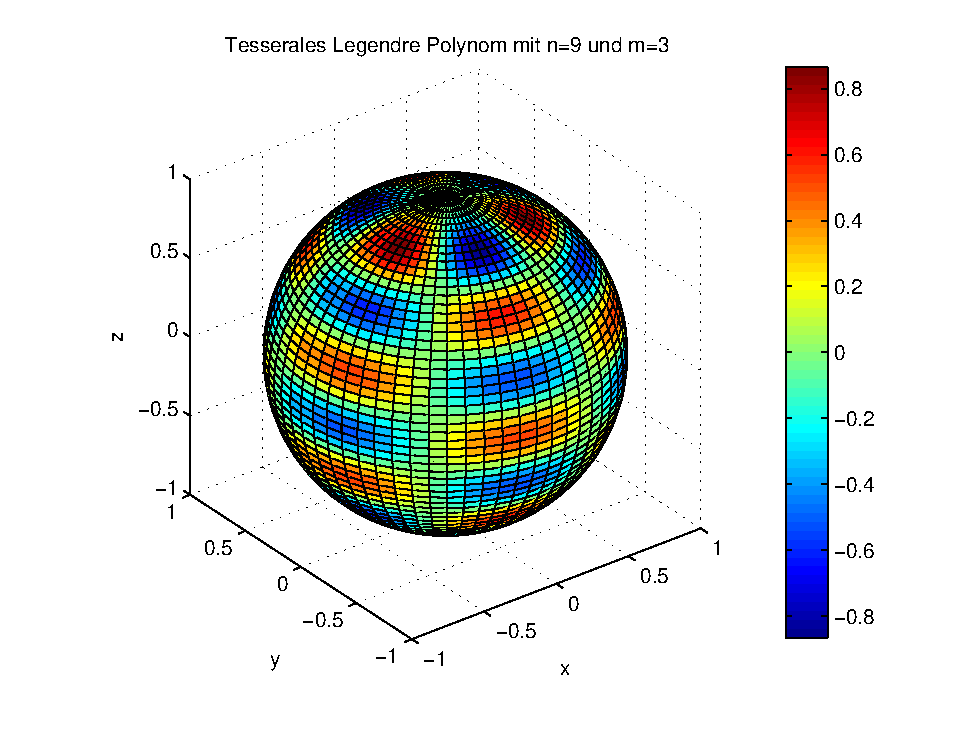
\includegraphics[scale=0.7]{tesseral.eps}
	\caption{Legendre-Polynom $P^{3}_{9}$ - tesseral}
	\end{center}
\end{figure}



\section{Aufgabenteil 2}
In dieser Aufgabe soll das Schwerefeld der Erde, welches beispielsweise aus Satellitenmessungen bekannt ist mittels der in Aufgabe 1 berechneten Legendre Polynome dargestellt werden. Die dazugeh�rigen Datens�tze zur Berechnung notwendiger Parameter haben wir der Institution des Helmholtz Centre Potsdam (GFZ German Research Centre For Geosciences) aus folgender Internetseite entnommen:\textit{http://icgem.gfz-potsdam.de/ICGEM}.\\
F�r die Aufgabenbearbeitung wurde das Datenfile \textit{osu89a.gfc} verwendet, welches die Koeffizienten der Kugelfunktionsentwicklung bis zu verschiedenen Graden und Ordnungen mit dazugeh�rigen Standardabweichungen enth�lt. Das Einlesen des Files erfolgte via load('osu.txt'). F�r die Berechnung des Potenzials ist zu beachten, dass die Koeffizienten der Polynome bis zum 10. Grad korrigiert werden (siehe Aufgabenblatt). Aufgrund der linearen Approximation des Potentials wird durch die Korrektur der Koeffizienten erreicht, dass die ersten Terme aus der Reihenentwicklung eine st�rkere Gewichtung erhalten, sodass ellipsoide Anteile (bzgl. des Referenzellipsoids) im Potentialfeld nicht �berwiegen und auch sehr geringe Anomalien zu erkennen sind. Das Programm zur Berechnung des Schwerepotentials ist folgend strukturiert:
\begin{itemize}
\item Einlesen des Datenfiles
\item Deklaration der Variablen
\item Anordnung der Koeffizienteneintr�ge in neue Matrizen $C_{nm}$ und $S_{nm}$ mit dazugeh�rigem Grad und Ordnung
\item Korrektur der Koeffizienten
\item Schleife �ber $\theta$ und $\Phi$
\item Berechnung der Legendre Polynome (+ Schmidt-Normalisierung)
\item Berechnung des Potenzials �ber Schleife (m,n) und Summenbildung
\item graphische Darstellung des Schwerepotentials
\end{itemize}
Eine detaillierte Beschreibung ist dem Programmcode im Anhang zu entnehmen.
Die Berechnung des Potenzials der Erde basiert auf folgendem Zusammenhang:
\begin{equation}
U_{g}= \frac{\gamma M}{r}\sum_{n=0}^{\infty}(\frac{a}{r})^n\sum_{m=0}^{n} P_{mn}(\theta)[C_{nm}\cos m\Phi + S_{nm}\sin m\Phi]
\end{equation}

Die zwei folgenden Abbildungen zeigen, dass variierende Ordnungen (n) der Legendre Polynome unterschiedliche Ergebnisse f�r das Schwerepotential liefern. Demnach bestimmt die H�he der Ordnungen n und damit die Anzahl berechneter Koeffizienten das Aufl�sungsverm�gen der zu ermittelnden Gr��e. Bei der Berechnung des Potentials mit n=200 werden auch kleinste Anomalien sichtbar, w�hrend f�r n=5 kleinskalige Undulationen nicht ber�cksichtigt werden. Dies ist auf die kurzwelligen Anteile der Koeffizienten zur�ckzuf�hren, welche durch eine hohe Ordnung der Kugelfl�chenfunktionen sichtbar beziehungsweise f�r Koeffizienten $n\leq 5$ unterdr�ckt werden.

\begin{figure}[h!]
	\center
	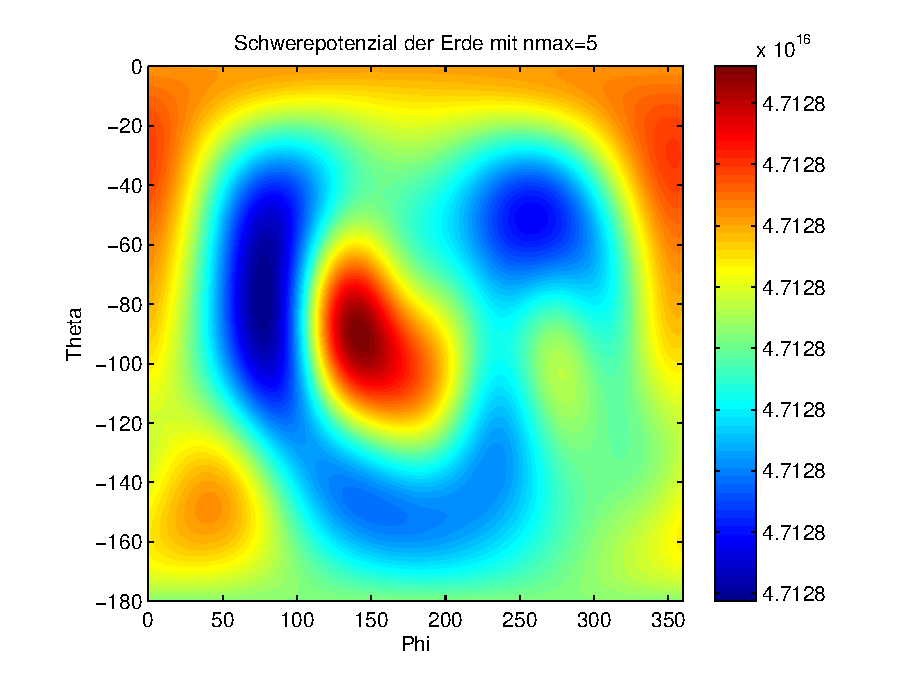
\includegraphics[scale=0.7]{nn5.eps}
	\caption{Das Schwerepotential f�r nmax=5 - sehr geringe Aufl�sung}
\end{figure}

\begin{figure}[h!]
	\center
	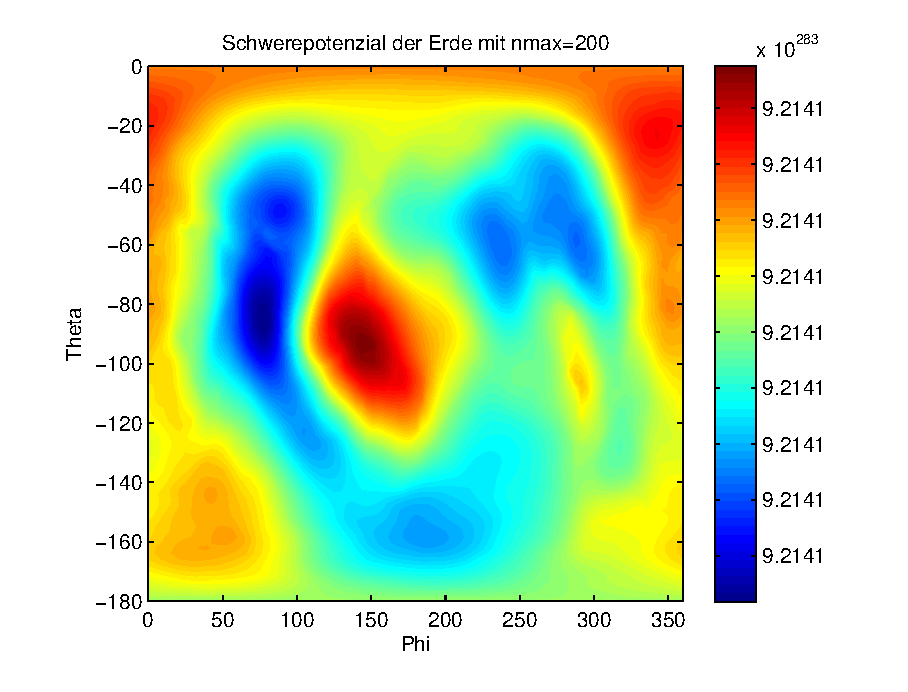
\includegraphics[scale=0.7]{nn200.eps}
	\caption{Das Schwerepotential f�r nmax=200 - geringe Anomalien sichtbar}
\end{figure}

In den anschlie�enden Abbildungen sind drei Auschnitte dargestellt die besonders starke Schwereanomalien aufweisen. Die Ursache f�r die langwelligen Anomalien sind auf gro�r�umige Dichtevariationen im Erdmantel beziehungsweise in der Erdkruste zur�ckzuf�hren. Eine h�here Gesteinsdichte erzeugt demnach eine zus�tzliche Gravitationsbeschleunigung, wodurch der Massen�berschuss eine positive Schwereanomalie bewirkt und das Geoid ''ausbeult''. Andererseits werden durch geringere Dichten negative Schwereanomalien verursacht die ''Eindellungen'' des Geoids hervorrufen. Die Dichtevariationen im Erdmantel werden durch die Geodynamik der Mantelkonvektion begr�ndet. Demnach weist extrem hei�es Mantelmaterial eine geringe Dichte auf und steigt nach oben, wogegen sich kalte Regionen durch eine hohe Dichte ausweisen und absinken. Folglich sind abtauchende Konvektionsstr�me urs�chlich f�r positive Schwereanomalien (Beulen) und aufsteigende Konvektionsstr�me verantwortlich f�r negative Anomalien (Dellen).\\
Auch die Topographie f�hrt zu lateral variablen Massenvariationen und f�hrt zu Schwereanomalien (siehe Abb.?? Himalaya)
bla bla beispiele:
%\chapter{Oberfl�chenstrukturen}
Die Oberfl�che des Mondes umfasst 38$km^{2}$ und zeichnet sich durch seine hemisph�rische Gegens�tzlichkeit zwischen der erabgewandten (far side) und erdzugewandten Seite (near side) aus.
So wird die erdzugewandte Seite des Mondes durch die Maria \textit{(Abb.1a)} charakterisiert, welche 31,2$\%$ dieser Fl�che einnehmen. Auf der erdabgewandten Seite sind hingegen die highlands \textit{(Abb.1b)} vorherrschend, die dort 45$\%$ der Oberfl�che bedecken.
Marias sind topographisch niedrige Gebiete, die auch als Tiefebenen bezeichnet werden. Dabei handelt es sich um fast ebene Fl�chen, die entstandene Impaktbecken aus der Fr�hzeit mit basaltischen Lavadecken verf�llt haben.
Die Krustenm�chtigkeit der near side mit maximal 60 km ist deutlich geringer als die der far side und beg�nstigt demensprechende Magmaaustritte an der Oberfl�che, wodurch sich die gr��ere Fl�chenbedeckung der Maria auf der erdzugewandten Seite begr�ndet.\\
Die durch Druckabgabe der Partialschmelzen gebildeten Mare-Basalte weisen anhand ihrer chemischen Zusammensetzung gro�e �hnlichkeiten mit den terrestrischen Basalten der ozeanischen Kruste auf. Das gr��te mit Mare-Basalten verf�llte Becken ist das Imbrium-Becken mit einer Fl�chenausdehung von 830.000 $km^{2}$ und einem Durchmesser von 1123 km im zentral-n�rdlichen Teil auf der near side.\\ 
Die Gegens�tzlichkeit der Maria auf der near side umfasst die auf der far side dominierenden highlands. In diesem Fall handelt es sich um topographisch erh�hte Gebiete die auf der einen Seite von mehreren hunderte Kilometer langen T�lern durchzogen sind und andererseits aus bis zu 10 km hohen Gebirgen bestehen. �ber die Entstehung der highlands existieren mehrere Theorien. Demnach handelt es sich um Reste von Kraterw�nden oder die Formation der highlands erfolgte durch die Komprimierung des Mondes w�hrend der Abk�hlungsphase, wodurch sich die Kruste an der Oberfl�che zu Faltengebirgen aufw�lbte. Die drei Hauptgesteinstypen der Highlands �hneln in ihrem Gef�ge den Plutoniten der Erde und umfassen Anorthosite, KREEP-Basalte \textit{(kristalline rare earth-elements)} und magnesiumreiche Gesteine die sich aus den Anorthositen bilden und �berwiegend mit Olivin und Pyroxen angereichert sind. Aus Isotopensystematiken von Mondanorthositen wurde ein Alter von etwa 4,4 Mrd. Jahren datiert. Dementsprechend stimmt die Altersdatierung der Highland-Gesteine mit dem Bildungsalter der ersten Kruste und dem Kristallisationszeitpunkt des urspr�nglichen Magmaozeans �berein.

%\input{Konvektion}
%\input{Zusammenfassung}
\cleardoublepage
%% Literaturverzeichnis %%%%%%%%%%%%%%%%%%%%%%%%%%%%%%%%%%%%%

%\headsep = 0.0 cm
%\pagenumbering{Roman}
%\bibliography{Literaturverzeichnis}
%\bibliographystyle{unsrtdin}
%\addcontentsline{toc}{chapter}{Literaturverzeichnis}
%\cleardoublepage
%%%%%%%%%%%%%%%%%%%%%%%%%%%%%%%%%%%%%%%%%%%%%%%%%%%%%%%%%%%%%
%% ANH�NGE
%%%%%%%%%%%%%%%%%%%%%%%%%%%%%%%%%%%%%%%%%%%%%%%%%%%%%%%%%%%%%

%\setcounter{page}{}

\begin{appendix}

\section{Quellcode}
\subsection{Aufgabe 1}
\lstinputlisting{aufg1.m}
%\newpage
%\subsection{Aufgabe 2}
%\lstinputlisting{Aufgabe2.m}
%\newpage
%\subsection{Aufgabe 3}
%\lstinputlisting{Aufgabe3.m}
\end{appendix}

\end{document}

